\section{Demo}
\begin{frame}
	\begin{center}
		{\fontsize{20}{20}\selectfont
			\textbf{DEMO}
		}
	\end{center}
\end{frame}

\begin{frame}
	\frametitle{N}
	\centering
	\begin{figure}
		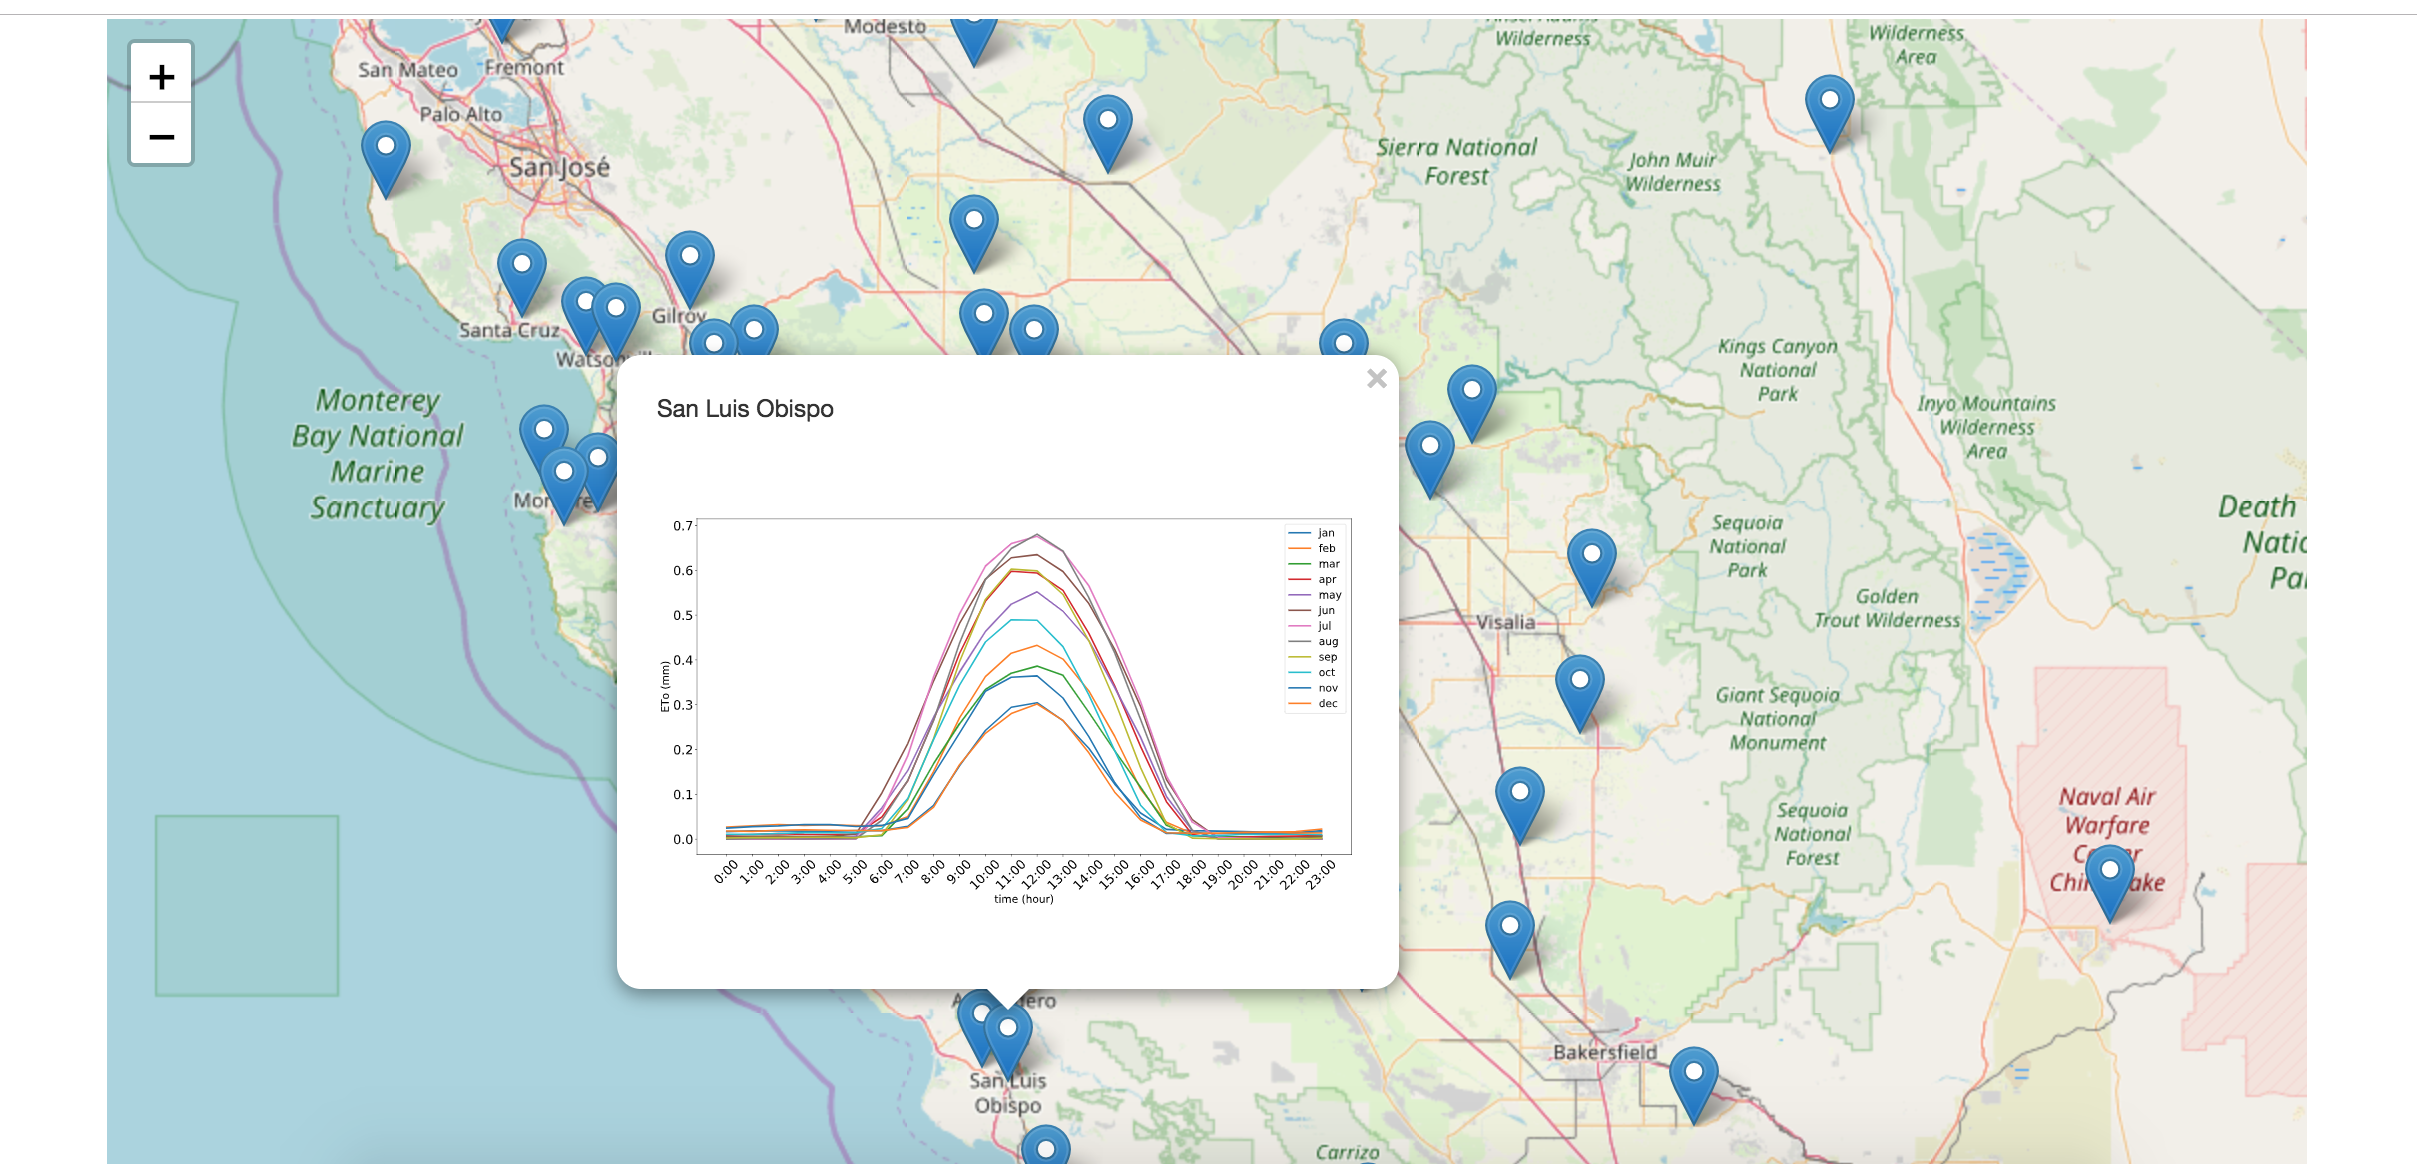
\includegraphics[width=0.9\textwidth]{images/fig1.png}
		\caption{N}\label{fig:2-2016}
	\end{figure}
\end{frame}

\begin{frame}
	\frametitle{N}
	\centering
	\begin{figure}
		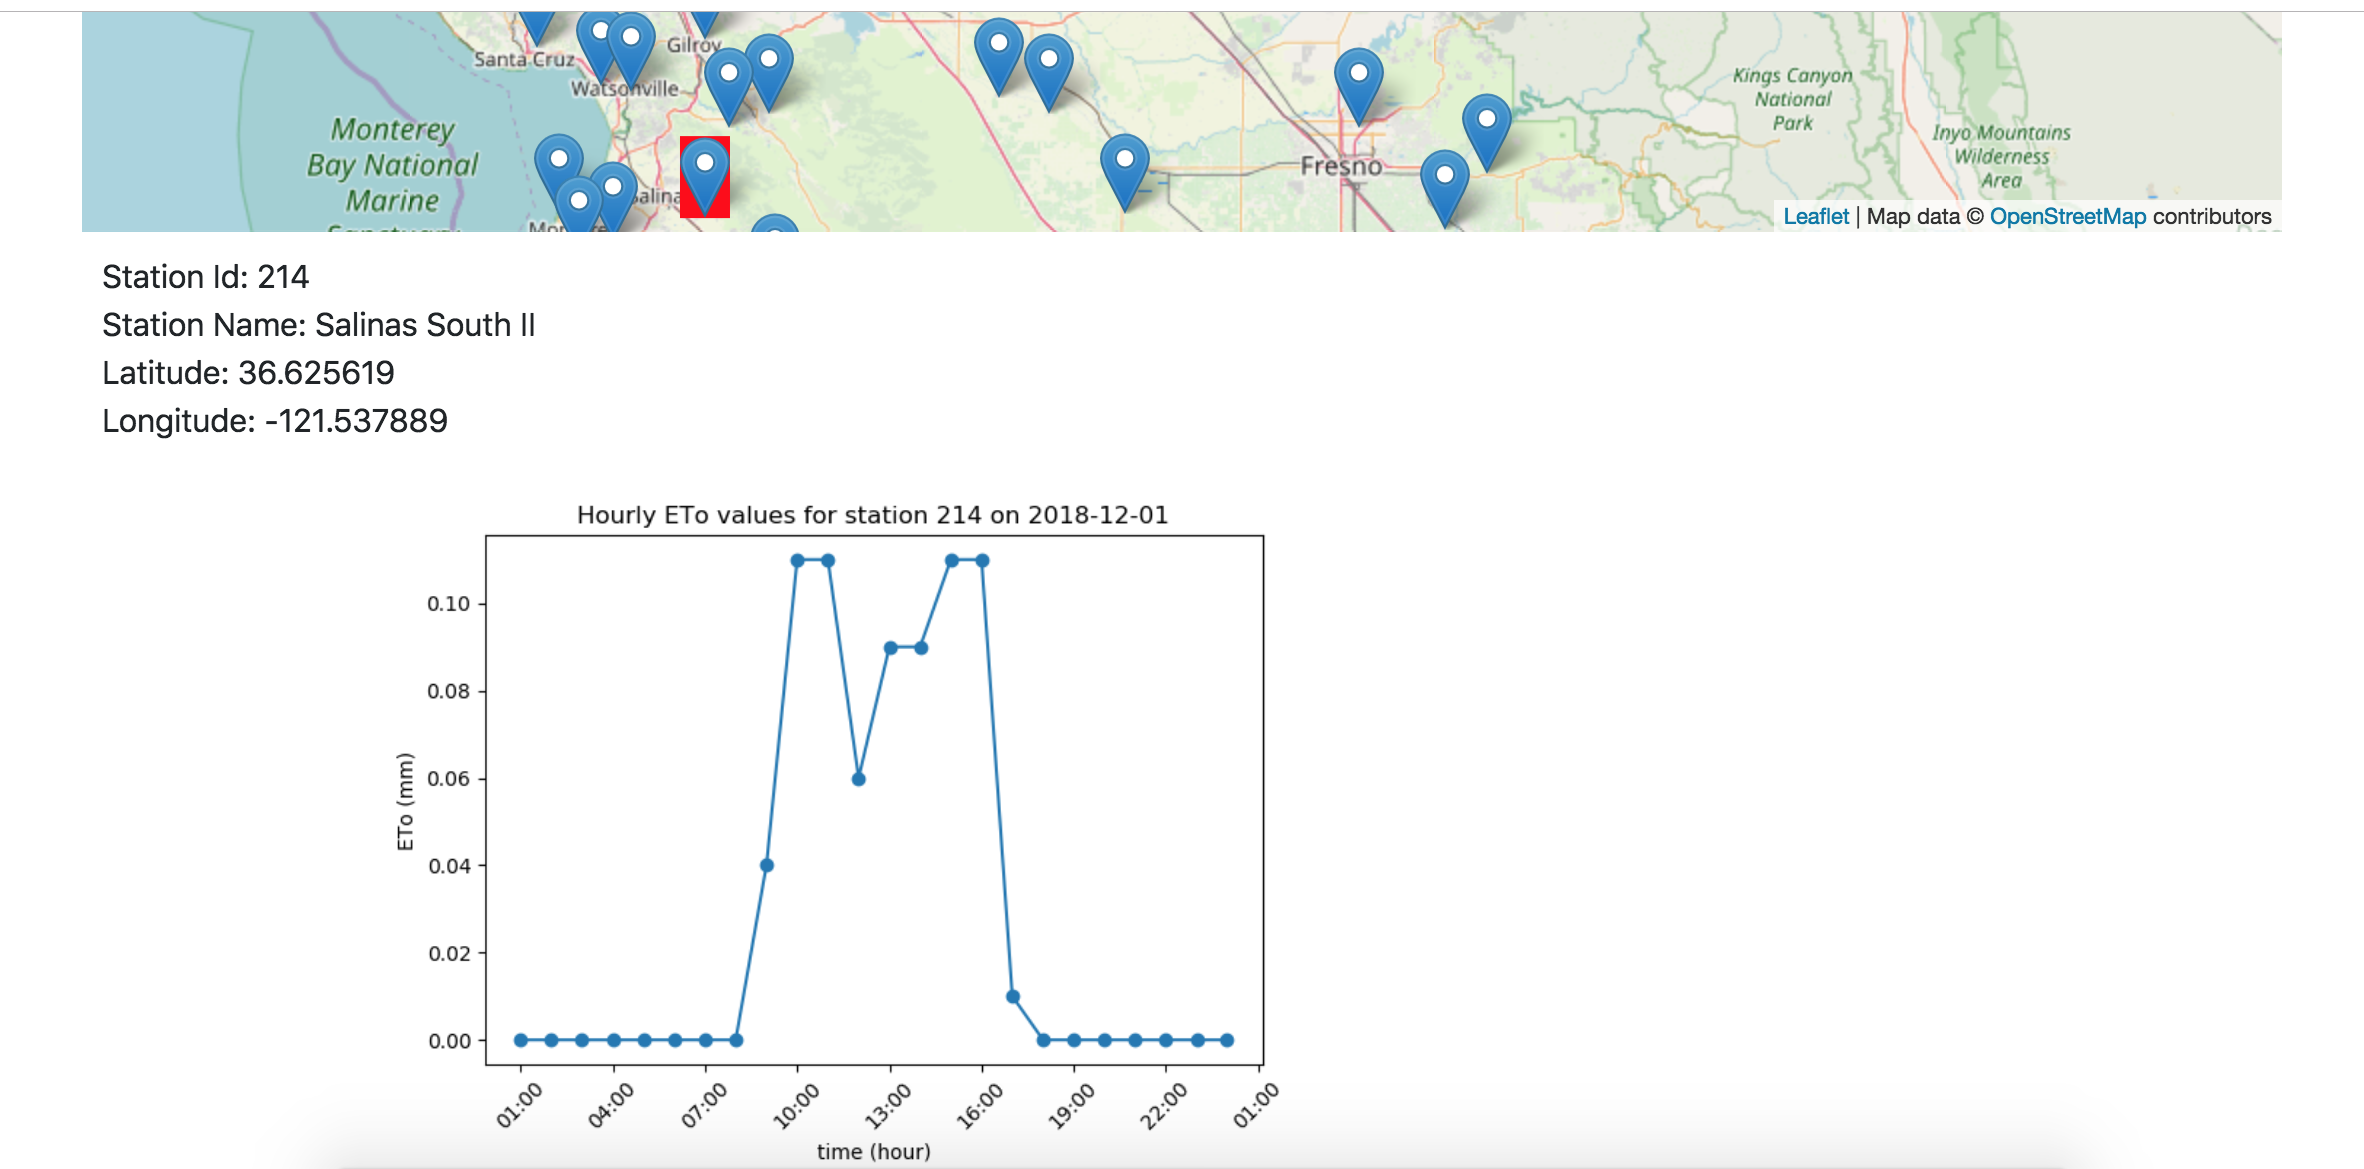
\includegraphics[width=0.9\textwidth]{images/fig2.png}
		\caption{N}\label{fig:2-2016}
	\end{figure}
\end{frame}

\begin{frame}
	\frametitle{N}
	\centering
	\begin{figure}
		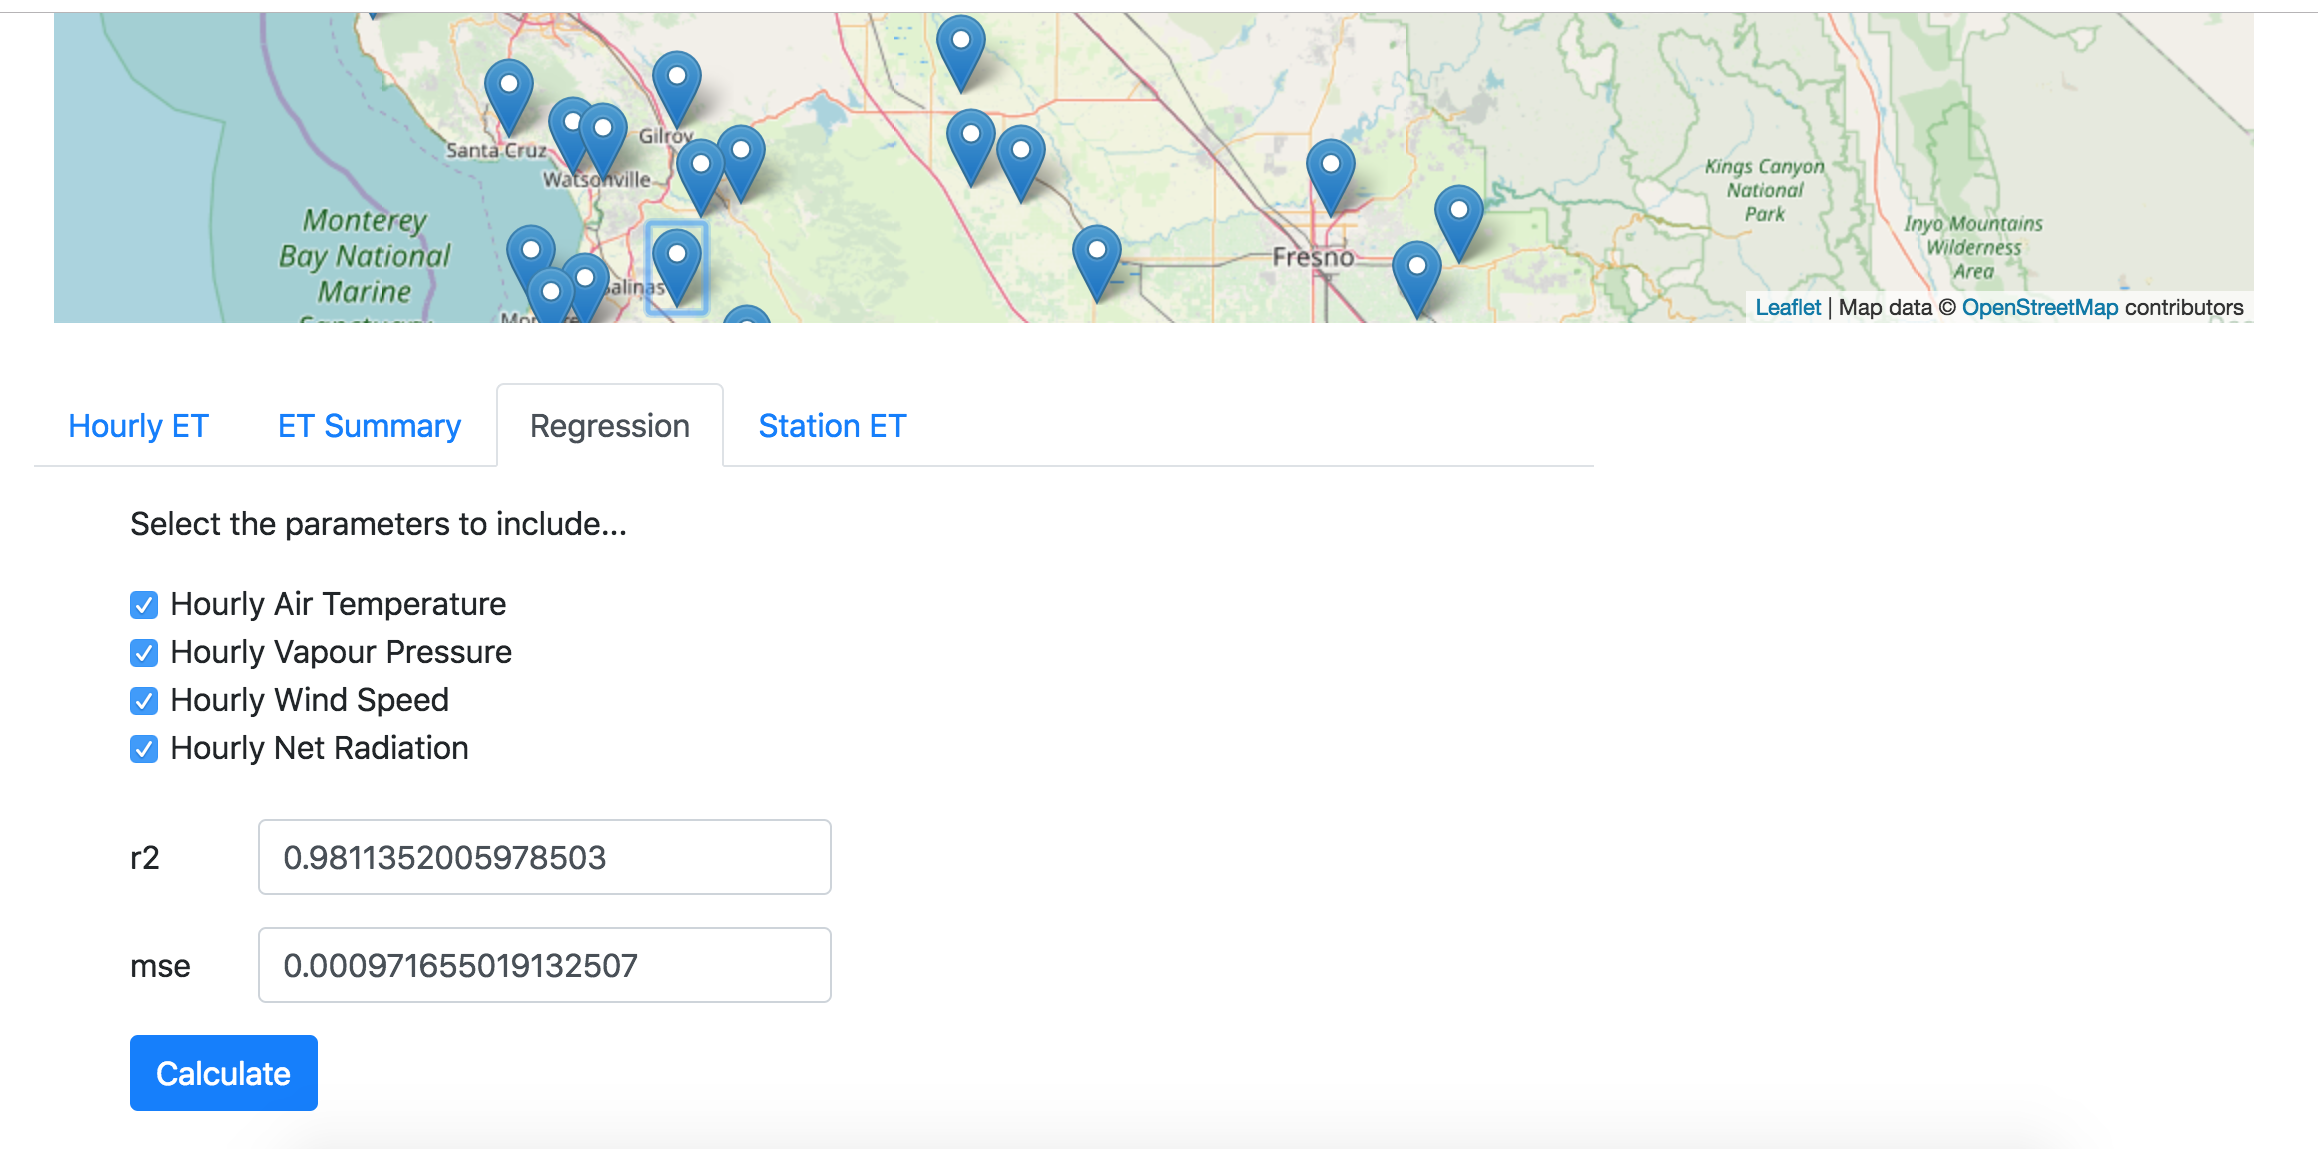
\includegraphics[width=0.9\textwidth]{images/fig3.png}
		\caption{N}\label{fig:2-2016}
	\end{figure}
\end{frame}

\begin{frame}
	In Fig.~\ref{fig:2-2016} we can see an example of the typical 12 month graph for one of the stations. There is a even spread between all the months in average hourly ET values and a smooth curve through the day. We can see that as we expected in the winter months ET values are lower than in the summer. There is a small amount of evapo-transpiration over the night which is not unusual but is not the case for all stations. 
\end{frame}

\begin{frame}
\frametitle{Normal 12-month Graph for Station 2 in 2016}
\centering
\begin{figure}
	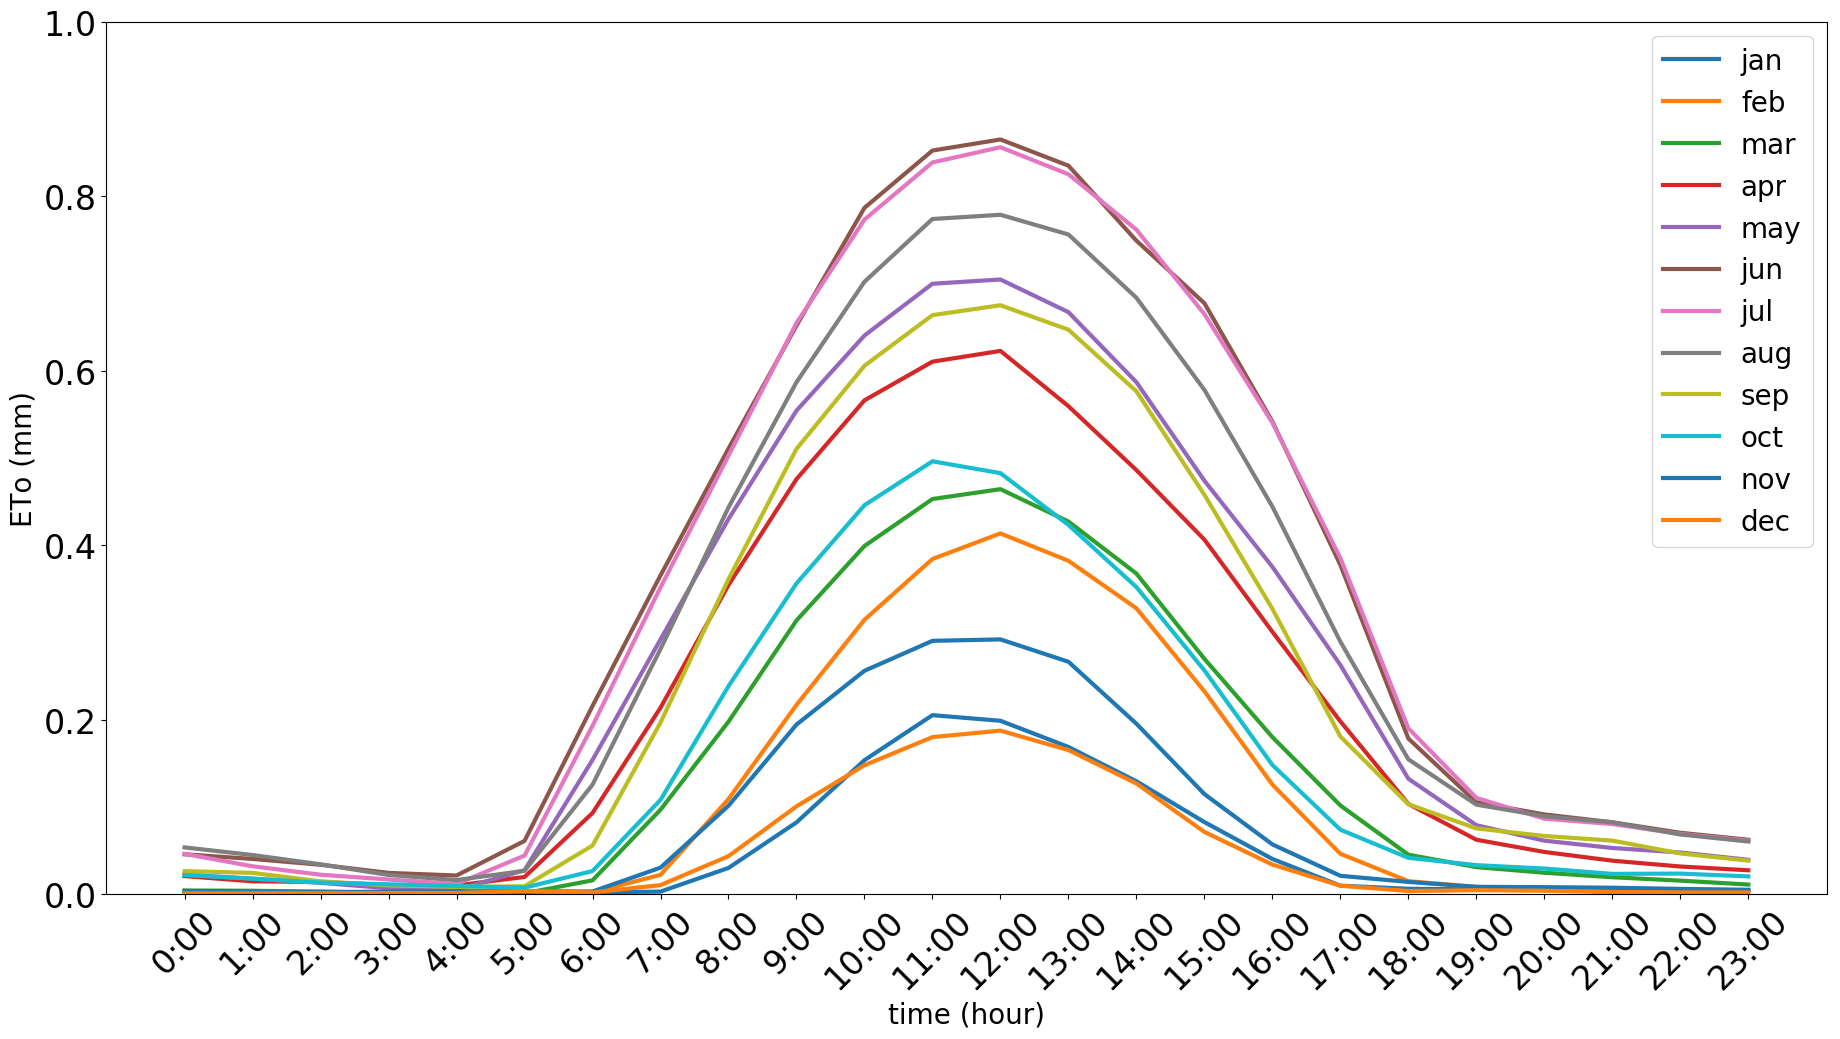
\includegraphics[width=0.9\textwidth]{images/2-2016.png}
	\caption{Normal 12-month Graph for Station 2 in 2016}\label{fig:2-2016}
\end{figure}
\end{frame}

\begin{frame}
	If we take a sampling of the all graphs produced from the many stations we see four different stations types. In Fig.~\ref{fig:12-2016} we see an example of the second category where there is a clear split between the winter and summer months. If we look at the graphs for stations like this through the years we can see that there is consistently a split between months but which months varies between years. In future work we could predict when this jump in ET values occurs to help farmers prepare to the increase in water needs. 
\end{frame}

\begin{frame}
\frametitle{12-month Graph for Station 12 in 2016}
\centering
\begin{figure}
	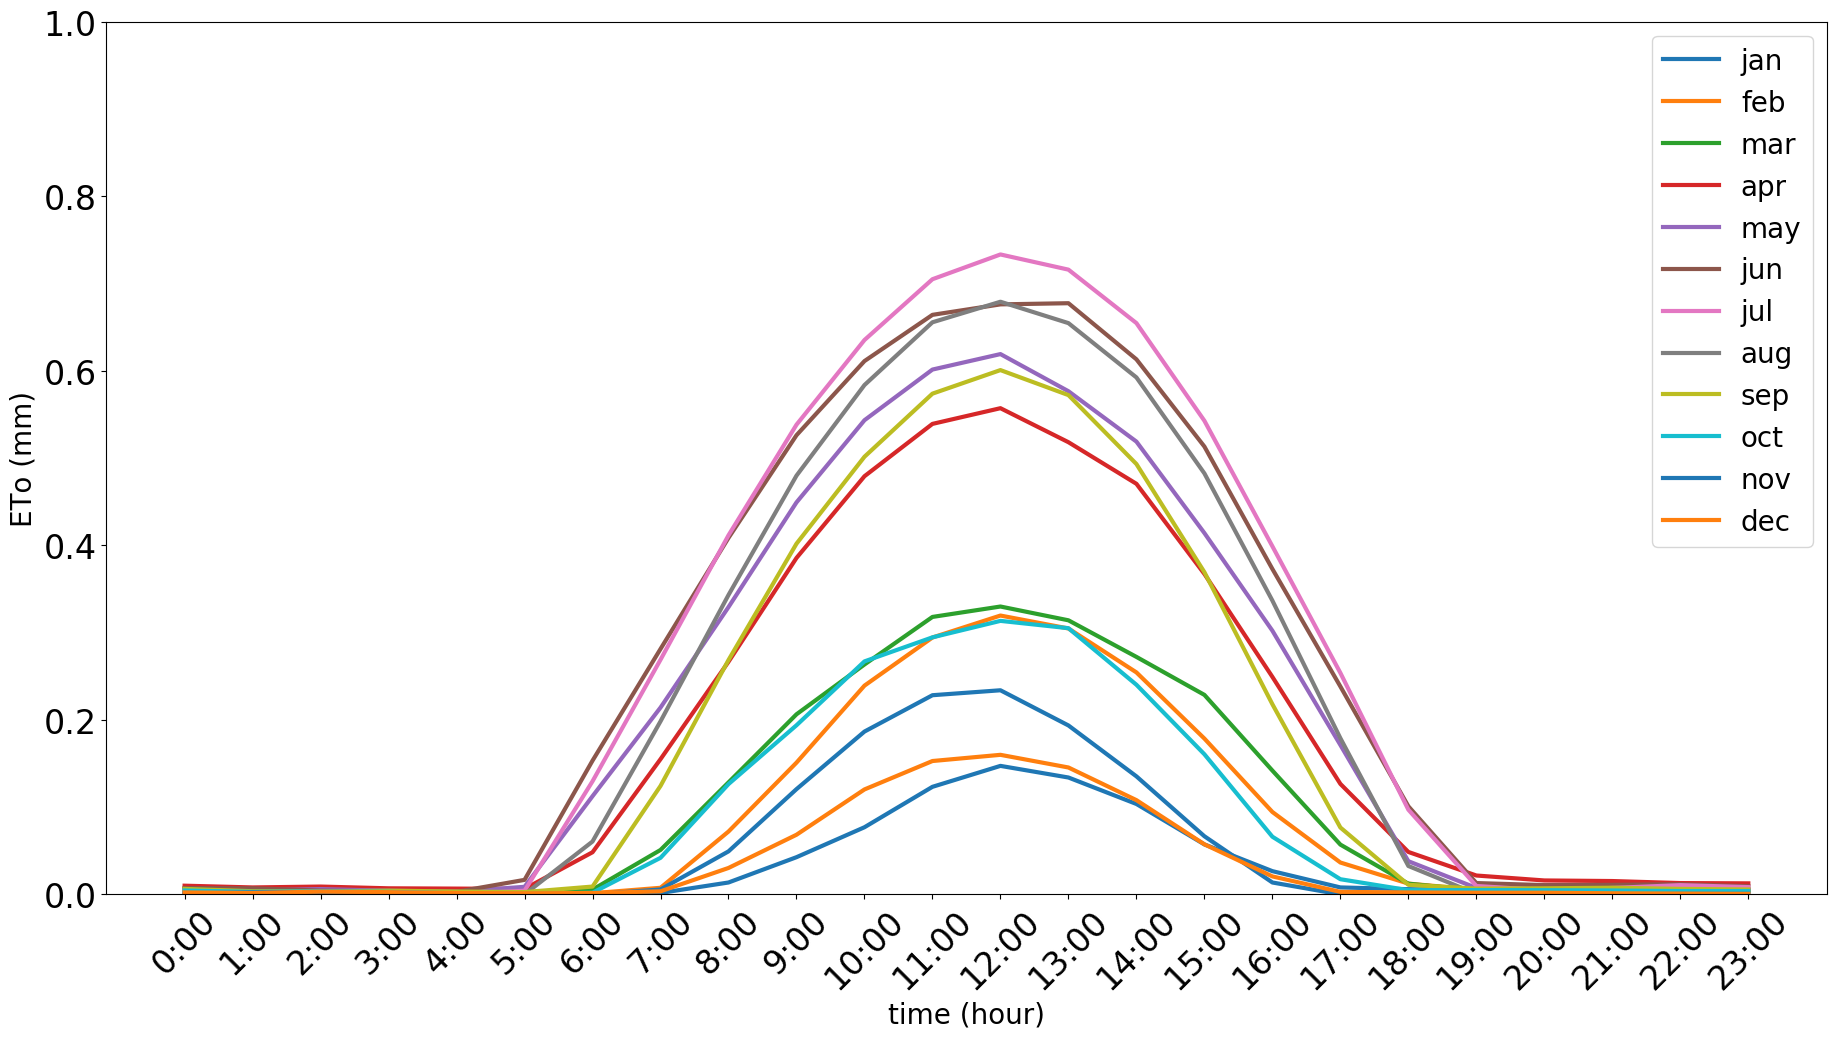
\includegraphics[width=0.9\textwidth]{images/12-2016.png}
	\caption{12-month Graph for Station 12 in 2016}\label{fig:12-2016}
\end{figure}
\end{frame}

\begin{frame}
	Here We can see an example (Fig.~\ref{fig:62-2018}) of an anomaly in the day where unexpectedly in the night the ET values start increasing. We don't know why this occurred but could be a sensor error or some large change in the local environment that cause ET to increase in the night.
\end{frame}

\begin{frame}
\frametitle{12-month Graph for Station 62 in 2018}
\centering
\begin{figure}
	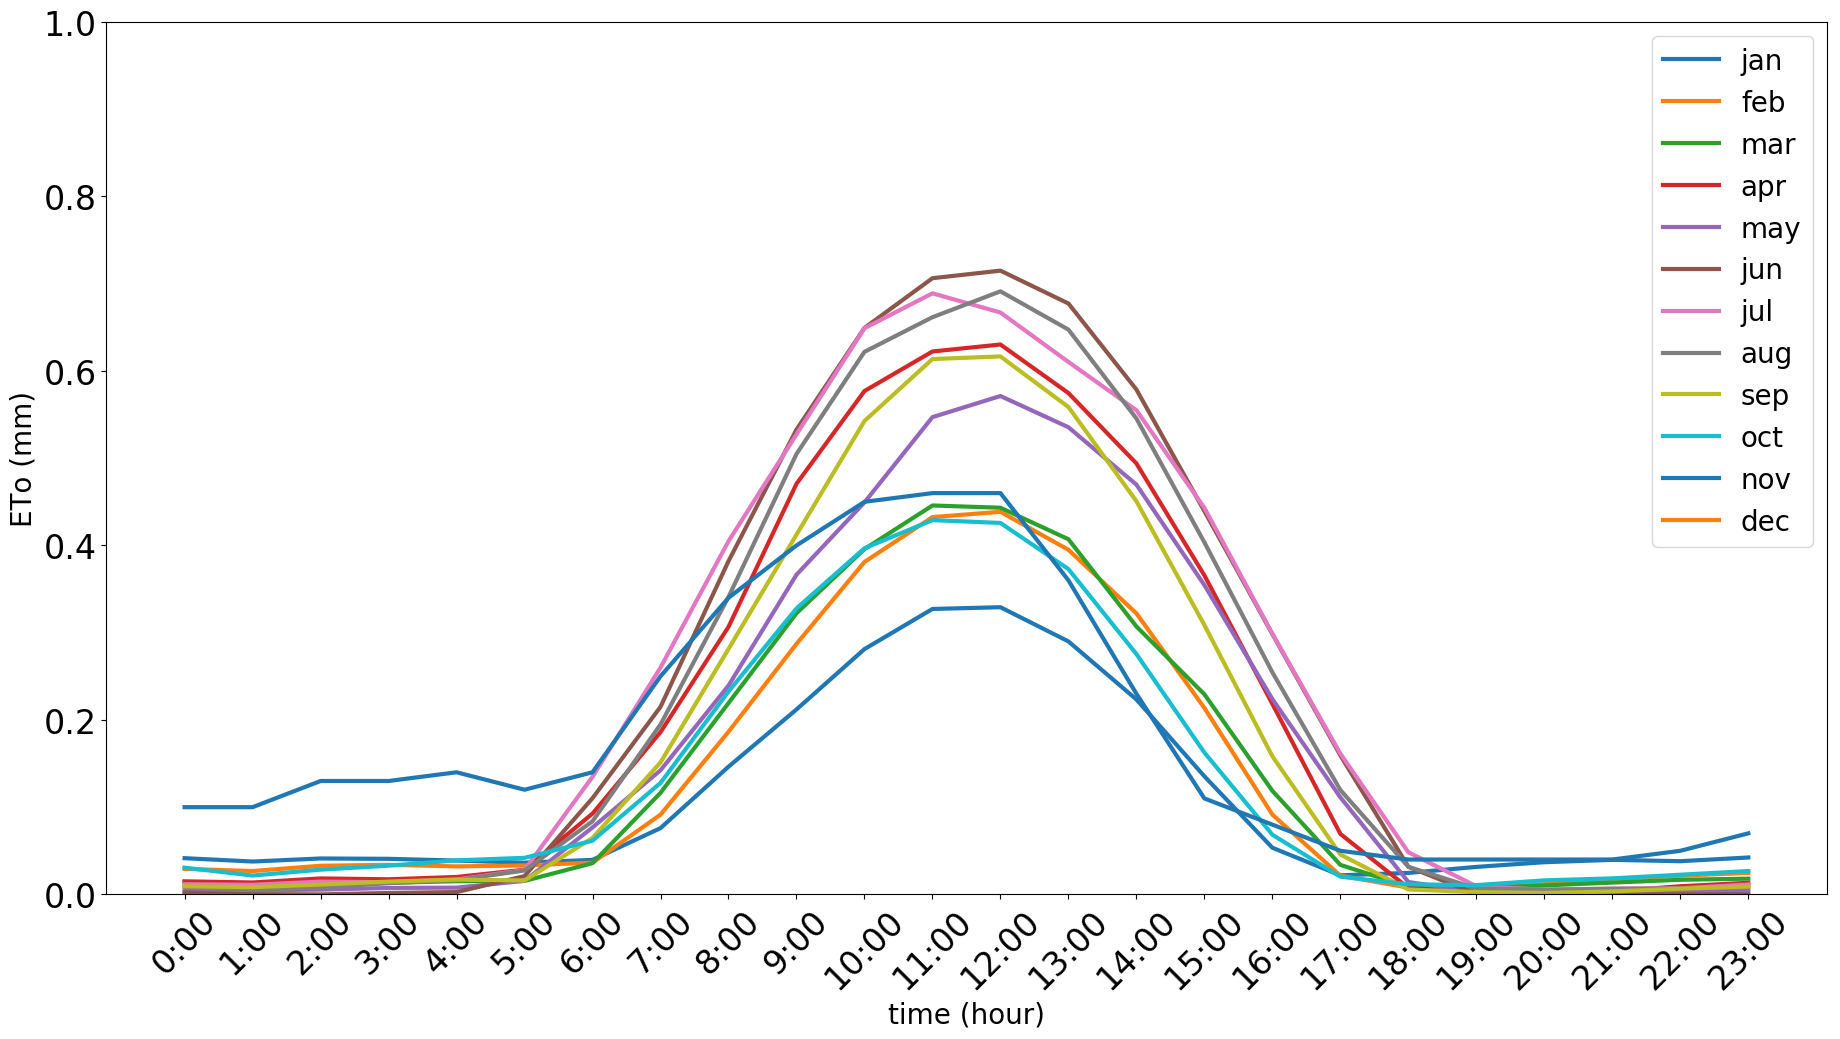
\includegraphics[width=0.9\textwidth]{images/62-2018.png}
	\caption{12-month Graph for Station 12 in 2016}\label{fig:62-2018}
\end{figure}
\end{frame}

\begin{frame}
	In Fig.~\ref{fig:234multi} we have a 3 year composite graph for 2016, 2017 and 2018. This particular station is an example of a location with a large tail of ET values that continues late into the night. We also see a trend where the ET values decrease between the years of 2016-2018. This could be an indication of a environmental that greatly reduced the water loss in the vicinity of that stations.
\end{frame}

\begin{frame}
\frametitle{36-month Graph for Station 234}
\centering
\begin{figure}
	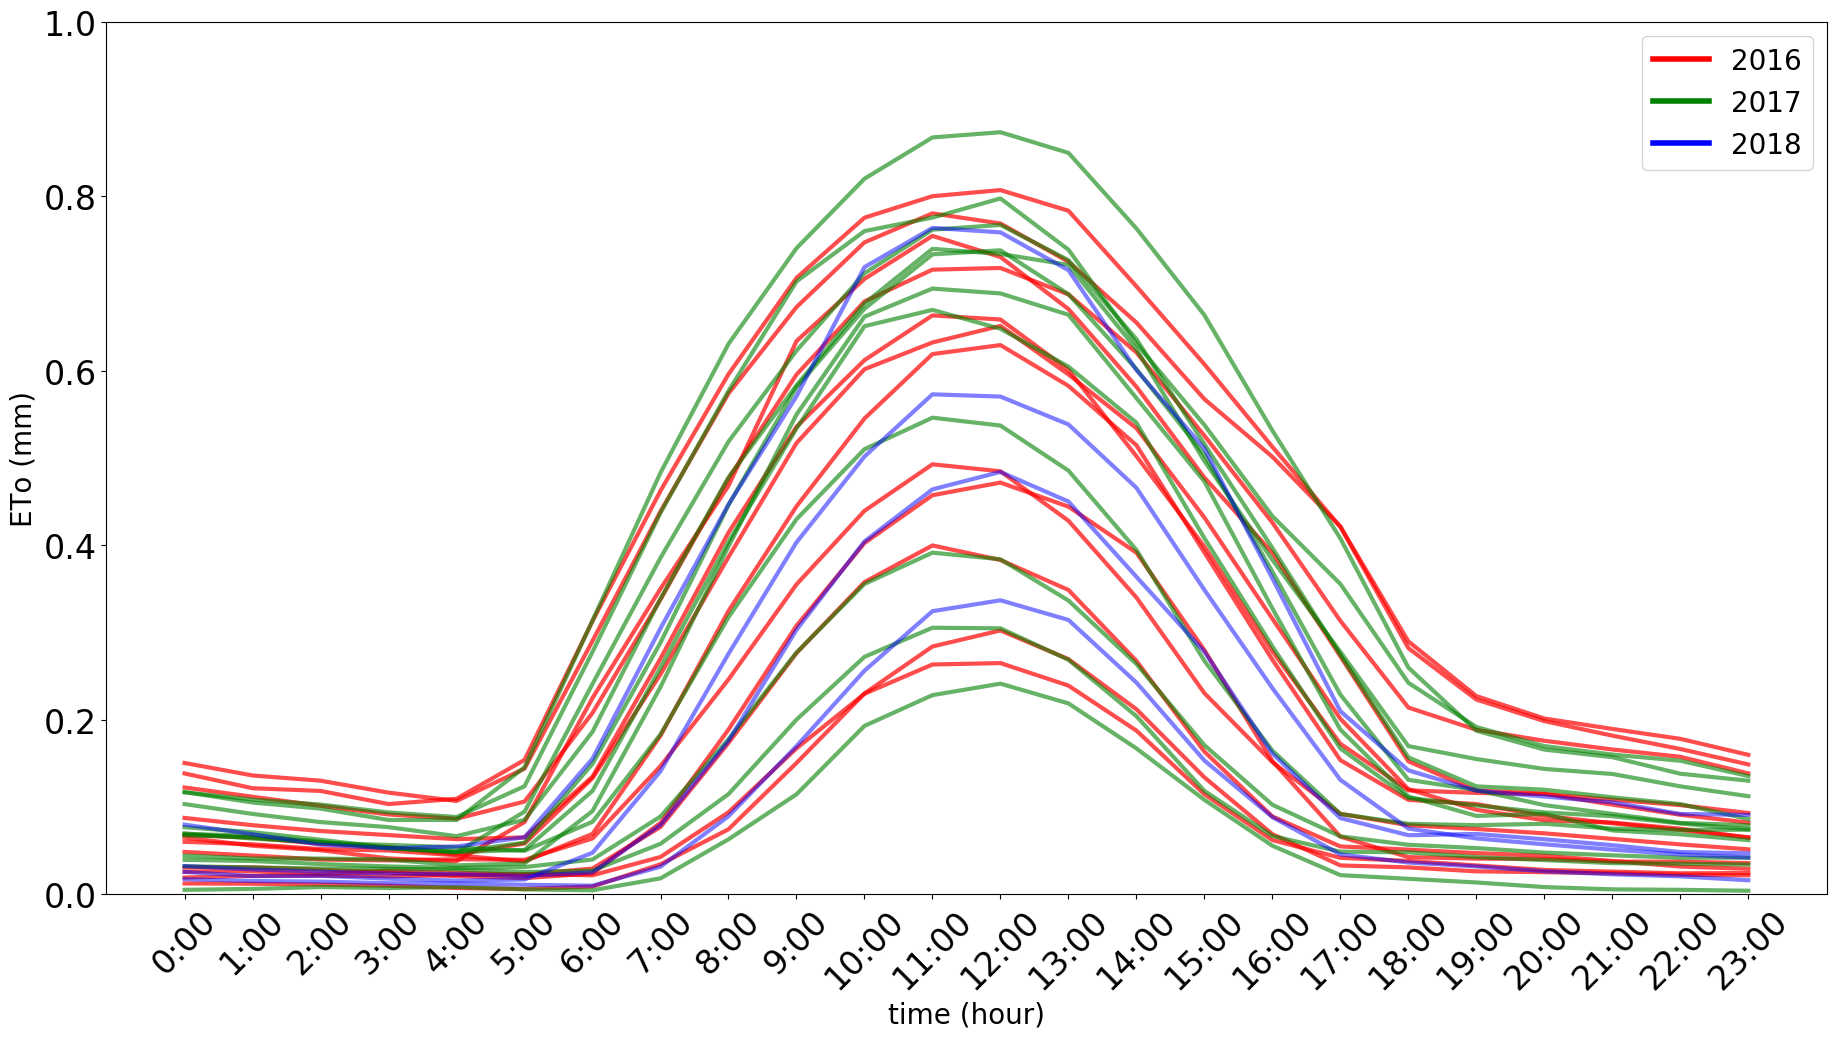
\includegraphics[width=0.9\textwidth]{images/234multi.png}
	\caption{36-month Graph for Station 234}\label{fig:234multi}
\end{figure}
\end{frame}

\begin{frame}
	Looking through the 3 years graphs for the stations we see an interesting trend for station 7 (Fig.~\ref{fig:7multi}). There is a dip in ET values during the winter months at 10am. We investigate the cause of this dip and we saw that there was a similar shape in the hourly solar radiation graph(Fig.~\ref{fig:solar}). Looking at the google maps location for stations 7 we can see that a tree would block the sensor in the winter when the sun is at a lower angle.
\end{frame}

\begin{frame}
\frametitle{36-month Graph for Station 7}
\centering
\begin{figure}
	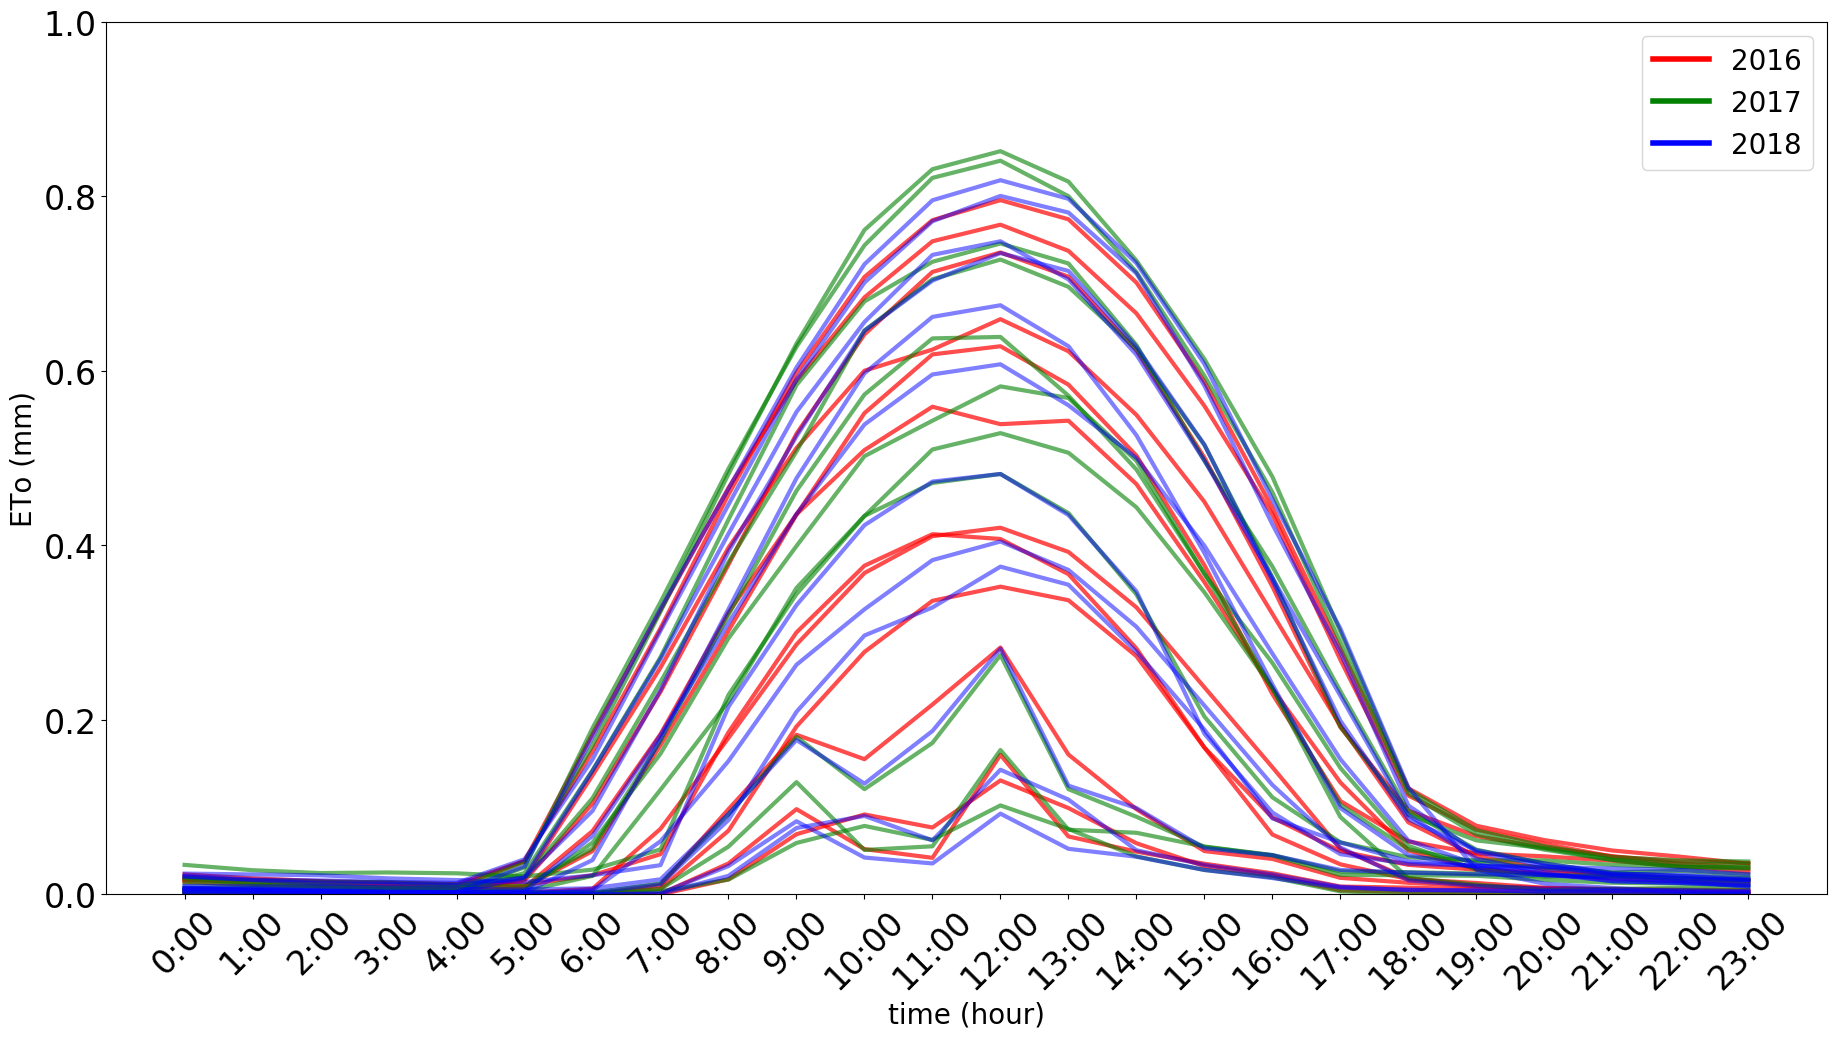
\includegraphics[width=0.9\textwidth]{images/7multi.png}
	\caption{36-month Graph for Station 7}\label{fig:7multi}
\end{figure}
\end{frame}


\begin{frame}
\frametitle{36-month Solar Graph for Station 7}
\centering
\begin{figure}
	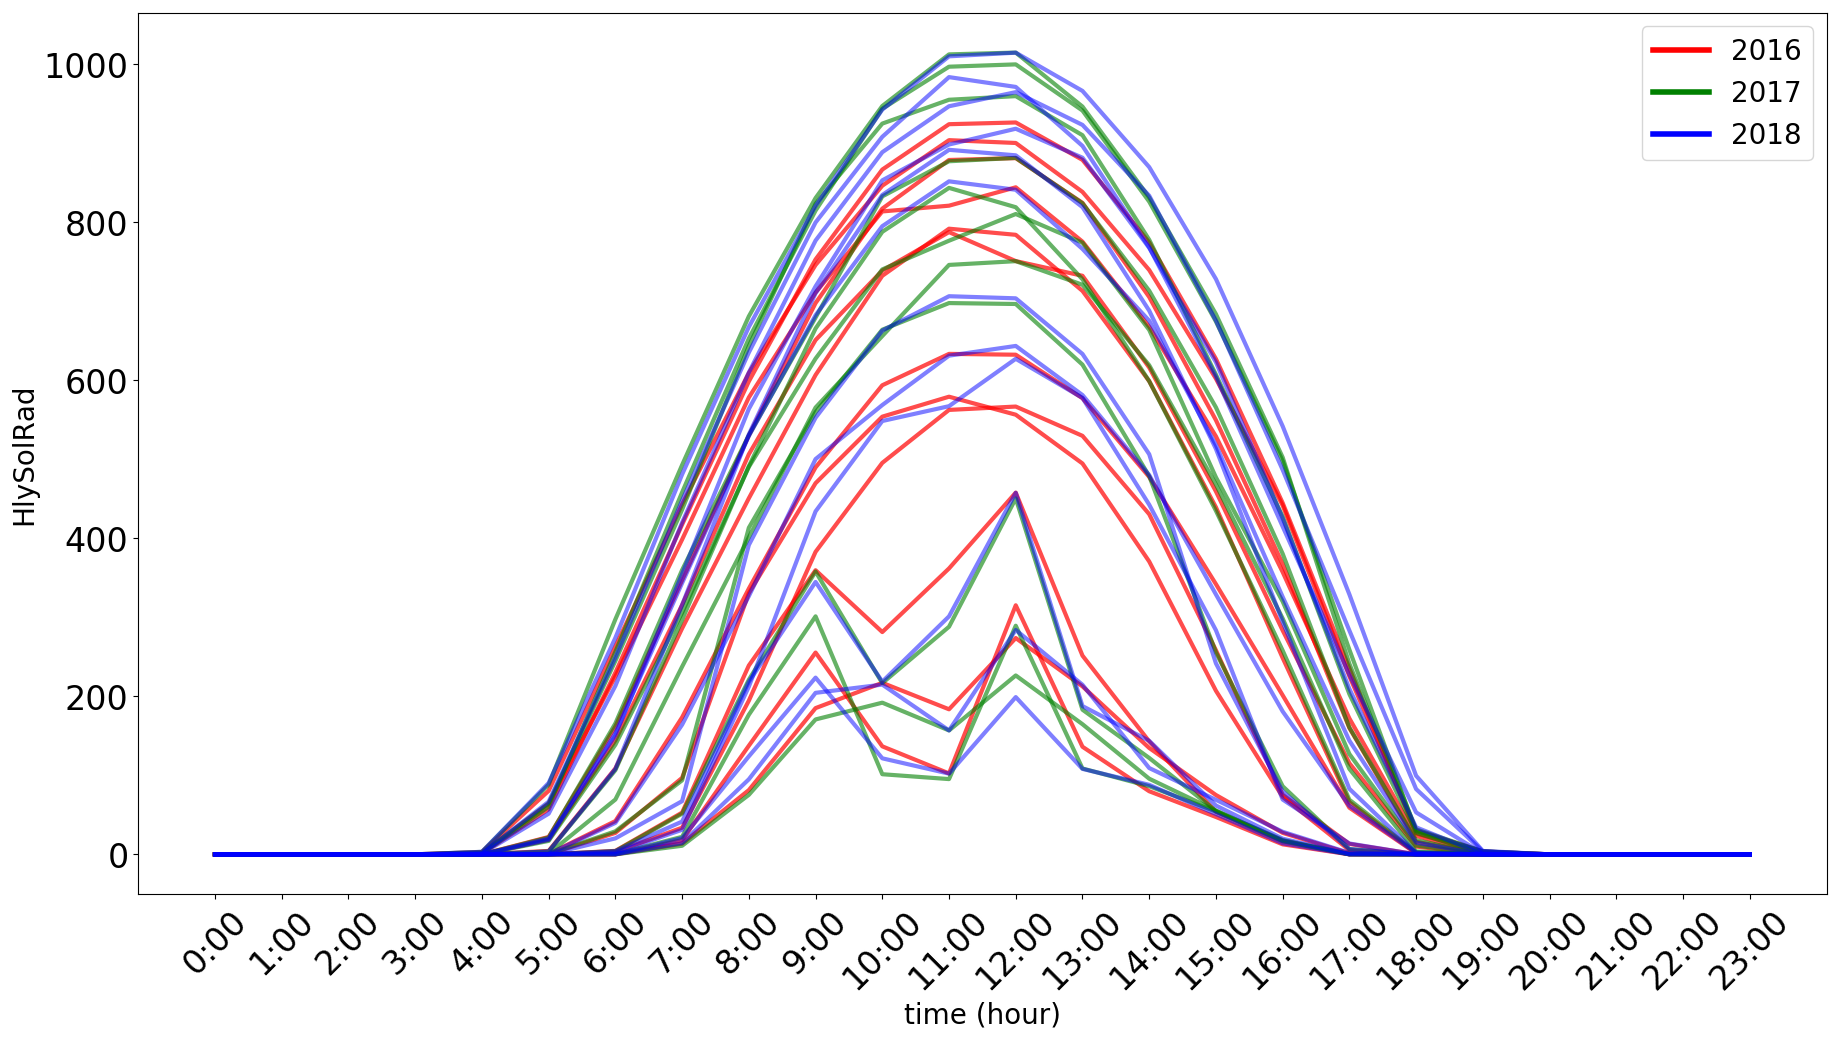
\includegraphics[width=0.9\textwidth]{images/3year7solar.png}
	\caption{36-month Solar Graph for Station 7}\label{fig:solar}
\end{figure}
\end{frame}

\begin{frame}
	In Fig.~\ref{fig:202multi} we can see a similar issue as we saw in Fig.~\ref{fig:7multi}. Knowing which stations have inaccurate data for certain time period could help future predictive model when we know what data we can trust.
\end{frame}

\begin{frame}
\frametitle{36-month Graph for Station 202}
\centering
\begin{figure}
	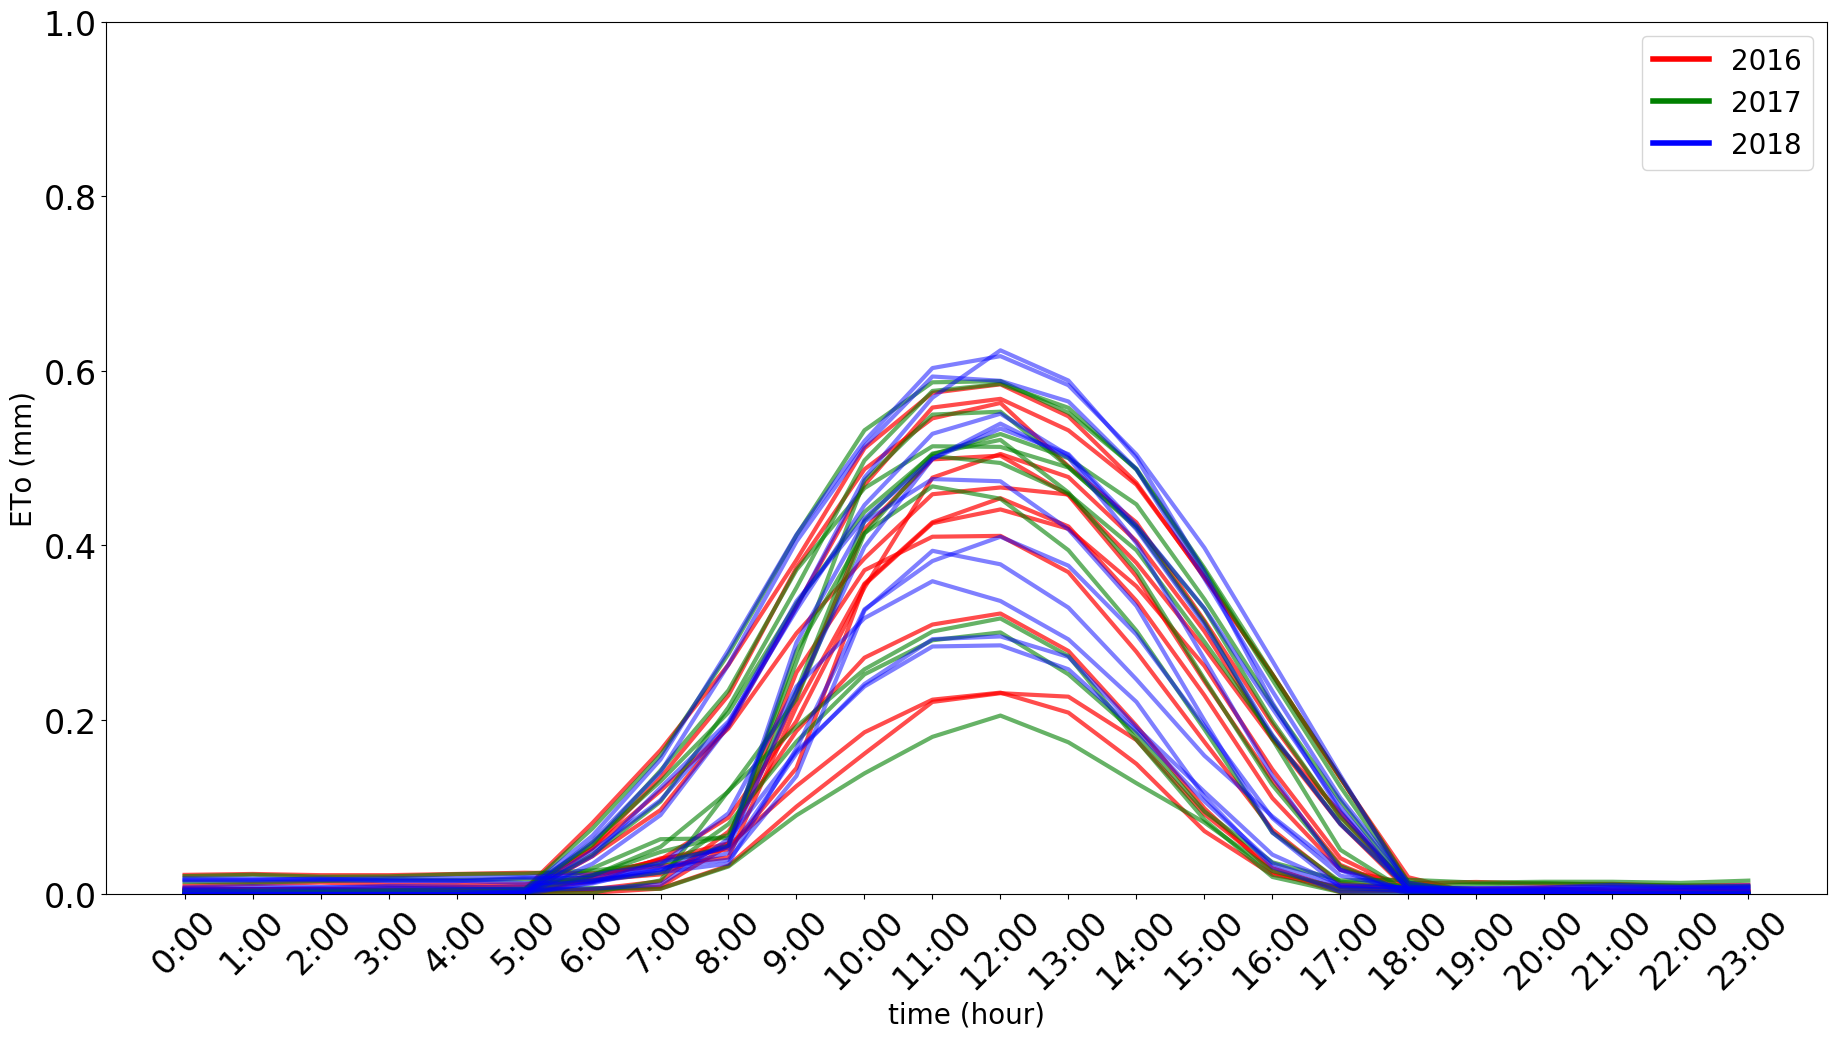
\includegraphics[width=0.9\textwidth]{images/202multi.png}
	\caption{36-month Graph for Station 202}\label{fig:202multi}
\end{figure}
\end{frame}

